% Options for packages loaded elsewhere
\PassOptionsToPackage{unicode}{hyperref}
\PassOptionsToPackage{hyphens}{url}
%
\documentclass[
]{book}
\usepackage{amsmath,amssymb}
\usepackage{lmodern}
\usepackage{ifxetex,ifluatex}
\ifnum 0\ifxetex 1\fi\ifluatex 1\fi=0 % if pdftex
  \usepackage[T1]{fontenc}
  \usepackage[utf8]{inputenc}
  \usepackage{textcomp} % provide euro and other symbols
\else % if luatex or xetex
  \usepackage{unicode-math}
  \defaultfontfeatures{Scale=MatchLowercase}
  \defaultfontfeatures[\rmfamily]{Ligatures=TeX,Scale=1}
\fi
% Use upquote if available, for straight quotes in verbatim environments
\IfFileExists{upquote.sty}{\usepackage{upquote}}{}
\IfFileExists{microtype.sty}{% use microtype if available
  \usepackage[]{microtype}
  \UseMicrotypeSet[protrusion]{basicmath} % disable protrusion for tt fonts
}{}
\makeatletter
\@ifundefined{KOMAClassName}{% if non-KOMA class
  \IfFileExists{parskip.sty}{%
    \usepackage{parskip}
  }{% else
    \setlength{\parindent}{0pt}
    \setlength{\parskip}{6pt plus 2pt minus 1pt}}
}{% if KOMA class
  \KOMAoptions{parskip=half}}
\makeatother
\usepackage{xcolor}
\IfFileExists{xurl.sty}{\usepackage{xurl}}{} % add URL line breaks if available
\IfFileExists{bookmark.sty}{\usepackage{bookmark}}{\usepackage{hyperref}}
\hypersetup{
  pdftitle={Outdoor Equity App Technical Documentation},
  pdfauthor={Clarissa Boyajian and Halina Do-Linh},
  hidelinks,
  pdfcreator={LaTeX via pandoc}}
\urlstyle{same} % disable monospaced font for URLs
\usepackage{color}
\usepackage{fancyvrb}
\newcommand{\VerbBar}{|}
\newcommand{\VERB}{\Verb[commandchars=\\\{\}]}
\DefineVerbatimEnvironment{Highlighting}{Verbatim}{commandchars=\\\{\}}
% Add ',fontsize=\small' for more characters per line
\usepackage{framed}
\definecolor{shadecolor}{RGB}{248,248,248}
\newenvironment{Shaded}{\begin{snugshade}}{\end{snugshade}}
\newcommand{\AlertTok}[1]{\textcolor[rgb]{0.94,0.16,0.16}{#1}}
\newcommand{\AnnotationTok}[1]{\textcolor[rgb]{0.56,0.35,0.01}{\textbf{\textit{#1}}}}
\newcommand{\AttributeTok}[1]{\textcolor[rgb]{0.77,0.63,0.00}{#1}}
\newcommand{\BaseNTok}[1]{\textcolor[rgb]{0.00,0.00,0.81}{#1}}
\newcommand{\BuiltInTok}[1]{#1}
\newcommand{\CharTok}[1]{\textcolor[rgb]{0.31,0.60,0.02}{#1}}
\newcommand{\CommentTok}[1]{\textcolor[rgb]{0.56,0.35,0.01}{\textit{#1}}}
\newcommand{\CommentVarTok}[1]{\textcolor[rgb]{0.56,0.35,0.01}{\textbf{\textit{#1}}}}
\newcommand{\ConstantTok}[1]{\textcolor[rgb]{0.00,0.00,0.00}{#1}}
\newcommand{\ControlFlowTok}[1]{\textcolor[rgb]{0.13,0.29,0.53}{\textbf{#1}}}
\newcommand{\DataTypeTok}[1]{\textcolor[rgb]{0.13,0.29,0.53}{#1}}
\newcommand{\DecValTok}[1]{\textcolor[rgb]{0.00,0.00,0.81}{#1}}
\newcommand{\DocumentationTok}[1]{\textcolor[rgb]{0.56,0.35,0.01}{\textbf{\textit{#1}}}}
\newcommand{\ErrorTok}[1]{\textcolor[rgb]{0.64,0.00,0.00}{\textbf{#1}}}
\newcommand{\ExtensionTok}[1]{#1}
\newcommand{\FloatTok}[1]{\textcolor[rgb]{0.00,0.00,0.81}{#1}}
\newcommand{\FunctionTok}[1]{\textcolor[rgb]{0.00,0.00,0.00}{#1}}
\newcommand{\ImportTok}[1]{#1}
\newcommand{\InformationTok}[1]{\textcolor[rgb]{0.56,0.35,0.01}{\textbf{\textit{#1}}}}
\newcommand{\KeywordTok}[1]{\textcolor[rgb]{0.13,0.29,0.53}{\textbf{#1}}}
\newcommand{\NormalTok}[1]{#1}
\newcommand{\OperatorTok}[1]{\textcolor[rgb]{0.81,0.36,0.00}{\textbf{#1}}}
\newcommand{\OtherTok}[1]{\textcolor[rgb]{0.56,0.35,0.01}{#1}}
\newcommand{\PreprocessorTok}[1]{\textcolor[rgb]{0.56,0.35,0.01}{\textit{#1}}}
\newcommand{\RegionMarkerTok}[1]{#1}
\newcommand{\SpecialCharTok}[1]{\textcolor[rgb]{0.00,0.00,0.00}{#1}}
\newcommand{\SpecialStringTok}[1]{\textcolor[rgb]{0.31,0.60,0.02}{#1}}
\newcommand{\StringTok}[1]{\textcolor[rgb]{0.31,0.60,0.02}{#1}}
\newcommand{\VariableTok}[1]{\textcolor[rgb]{0.00,0.00,0.00}{#1}}
\newcommand{\VerbatimStringTok}[1]{\textcolor[rgb]{0.31,0.60,0.02}{#1}}
\newcommand{\WarningTok}[1]{\textcolor[rgb]{0.56,0.35,0.01}{\textbf{\textit{#1}}}}
\usepackage{longtable,booktabs,array}
\usepackage{calc} % for calculating minipage widths
% Correct order of tables after \paragraph or \subparagraph
\usepackage{etoolbox}
\makeatletter
\patchcmd\longtable{\par}{\if@noskipsec\mbox{}\fi\par}{}{}
\makeatother
% Allow footnotes in longtable head/foot
\IfFileExists{footnotehyper.sty}{\usepackage{footnotehyper}}{\usepackage{footnote}}
\makesavenoteenv{longtable}
\usepackage{graphicx}
\makeatletter
\def\maxwidth{\ifdim\Gin@nat@width>\linewidth\linewidth\else\Gin@nat@width\fi}
\def\maxheight{\ifdim\Gin@nat@height>\textheight\textheight\else\Gin@nat@height\fi}
\makeatother
% Scale images if necessary, so that they will not overflow the page
% margins by default, and it is still possible to overwrite the defaults
% using explicit options in \includegraphics[width, height, ...]{}
\setkeys{Gin}{width=\maxwidth,height=\maxheight,keepaspectratio}
% Set default figure placement to htbp
\makeatletter
\def\fps@figure{htbp}
\makeatother
\setlength{\emergencystretch}{3em} % prevent overfull lines
\providecommand{\tightlist}{%
  \setlength{\itemsep}{0pt}\setlength{\parskip}{0pt}}
\setcounter{secnumdepth}{5}
\usepackage{booktabs}
\ifluatex
  \usepackage{selnolig}  % disable illegal ligatures
\fi
\usepackage[]{natbib}
\bibliographystyle{plainnat}

\title{Outdoor Equity App Technical Documentation}
\author{Clarissa Boyajian and Halina Do-Linh}
\date{2022-06-02}

\begin{document}
\maketitle

{
\setcounter{tocdepth}{1}
\tableofcontents
}
\hypertarget{about}{%
\chapter{About}\label{about}}

\hypertarget{abstract}{%
\section{Abstract}\label{abstract}}

Outdoor recreation and access to nature have well-documented positive impacts on mental and physical well-being. Federal public land management agencies in the United States offer a variety of outdoor recreation activities to visitors. However, people from different socioeconomic and identity groups access federal public lands unequally due to historical discrimination and current inequities. This project uses data from the \href{https://ridb.recreation.gov/landing}{Recreation Information Database (RIDB)} and the \href{https://www.census.gov/data.html}{United States Census Bureau (US Census)} to explore patterns of visitor use of reservable overnight sites (such as campgrounds, cabins, hike-in, and more). Specifically, we used 2018 reservation data and US Census data from the next available year to 2018 (i.e.~2018 median income data, 2015 language data). We created the interactive \href{https://shinyapps.bren.ucsb.edu/oe_app/}{Outdoor Equity App} that gives users tools to summarize data, explore relationships between RIDB and US Census variables, view maps of where visitors are coming from for reservable sites in California, and download subset data. This technical documentation includes information on metadata, application maintenance, and next steps for expanding the app to include visitor data from more locations and time periods.

\hypertarget{about-the-authors}{%
\section{About the Authors}\label{about-the-authors}}

This technical documentation for the \href{https://shinyapps.bren.ucsb.edu/oe_app/}{Outdoor Equity App} was created by \href{https://cboyajian.github.io/}{Clarissa Boyajian} and \href{https://hdolinh.github.io/}{Halina Do-Linh}. The app was created as the final \href{https://bren.ucsb.edu/projects/visualizing-visitor-use-trends-california-campsites-explore-equitable-access}{capstone project} for their \href{https://bren.ucsb.edu/masters-programs/master-environmental-data-science}{Master of Environmental Data Science} degrees from the University of California's \href{https://bren.ucsb.edu/}{Bren School of Environmental Science \& Management}. Both women are passionate about environmental justice, open science, the art of data visualizations, and spending time recreating outdoors. Please reach out to either of both of us with any questions.

This project could not have been completed without the support and guidance of the Bren School advisors \href{https://bren.ucsb.edu/people/frank-davis}{Dr.~Frank Davis} and \href{https://bren.ucsb.edu/people/allison-horst}{Dr.~Allison Horst} and our external advisors \href{https://gaynorlab.weebly.com/people.html}{Dr.~Kaitlyn Gaynor} and \href{https://www.willrice.us/}{Dr.~Will Rice}.

\hypertarget{helpful-links-and-resources}{%
\section{Helpful Links and Resources}\label{helpful-links-and-resources}}

The \href{https://shinyapps.bren.ucsb.edu/oe_app/}{Outdoor Equity App} is was created with the \texttt{shiny} package \citep{R-shiny} using RStudio version 1.4.1717-3. This technical documentation is hosted using GitHub Pages. The GitHub repository containing all code relating to this technical documentation can be found \href{https://github.com/cboyajian/outdoor-equity-tech-doc}{here} and the GitHub repository containing all code relating to Outdoor Equity App can be found \href{https://github.com/outdoor-equity/outdoor-equity}{here}.

\hypertarget{executive-summary}{%
\chapter{Executive Summary}\label{executive-summary}}

Outdoor recreation and access to nature have well-documented positive impacts on mental physical well-being. Federal public land management agencies in the United States offer a wide variety of activities to visitors. However, people from different socioeconomic and identity groups access federal public lands unequally due to historical discrimination and current inequities. The multi-agency program, Recreation One Stop (R1S), oversees the operations of \href{https://www.recreation.gov/}{Recreation.gov} and aims to increase access to recreation by providing online resources about nationwide recreational opportunities, allowing visitors to make reservations, and making the associated data accessible to all. The rich data on visitors that R1S collects presents an opportunity for the creation of more robust data-driven analytical tools to understand the patterns and correlations of this unequal access across the country and within individual recreation areas. Decision-makers can use these tools to explore and visualize how recreational opportunities on federal public lands are accessed.

Our overarching objective is to design and built an interactive web application that allows users to analyze patterns in the access and demand of visitors at reservable overnight sites (such as campgrounds, cabins, hike-in, and more), using data from the \href{https://ridb.recreation.gov/landing}{Recreation Information Database (RIDB)} and the \href{https://www.census.gov/data.html}{United States Census Bureau (US Census)}. These analyses will allow federal public land managers to explore relationships among attributes of recreation opportunities, reservation practices, and socioeconomic data from the regions of visitor origin. We achieved this goal through the creation of an interactive web application, the \href{https://shinyapps.bren.ucsb.edu/oe_app/}{Outdoor Equity App}, that allows for a wide range of visualization, metadata documentation, and subset data downloads. This technical documentation serves to document the Outdoor Equity App creation process, include information for ongoing maintenance, and provide suggestions for future use and expansion.

The app - which is implemented using the R programming language - accesses public RIDB and US Census data via direct download and application programming interfaces (API). All data and R code scripts are stored on the UCSB Taylor Server and version-controlled through GitHub. We isolated necessary variables and defined, standardized, and aggregated values in the data cleaning process. We calculated additional derived variables for each reservation, such as distance traveled and booking window, and summary statistics (e.g., mean and median) for census data at the ZIP code level. A data set that combines the US Census and RIDB data based on visitors' home ZIP code is the foundation for the Outdoor Equity App. We visualized distributions of variables and relationships between them with simple, straightforward figures. Within the app, users can subset the data to a specific overnight reservable site and visualize the distribution of a single variable, the relationship between two variables, or the visitorshed map (i.e.~area from where visitors are coming) for the selected site. The app currently only includes data for California reservable sites in fiscal year 2018 due to project scope limitations.

Throughout the analysis and app creation processes, external advisors and federal public land managers have reviewed and tested the Outdoor Equity App. We incorporated feedback into all parts of the processes to ensure our data, analysis, and final products are robust. Potential future updates to the Outdoor Equity App are discussed in this technical documentation and include temporal and spatial expansions and app maintenance. The temporal expansion would include cleaning additional datasets for years from 2012 to 2021 as well as expanding the app's interface to allow for temporal selections when subsetting data. The spatial expansion would focus on updating the app structure and server hosting capabilities so the app runs smoothly with data from the full United States.

As environmental justice is increasingly recognized as a necessary lens to achieve environmental goals, equitable access to outdoor recreation is a high priority for managers. This tool assists managers to be equity-conscious decision-makers, can be a springboard for researchers who have questions about outdoor recreation, and strengthens nonprofit organizations' advocacy efforts. We also hope it will be a dynamic tool that empowers visitors to access the information and resources they need to explore outdoor recreation.

\hypertarget{problem-statement}{%
\chapter{Problem Statement}\label{problem-statement}}

\hypertarget{background}{%
\section{Background}\label{background}}

Outdoor recreation provides critical health and well-being benefits to communities, and in the United States, federal public lands play an important role in providing access to nature. However, access is not equal for all people \citep{Ewert1990}; \citep{Flores2018}, which has been recognized as an environmental injustice \citep{Floyd2002}. Many studies have shown that federally managed public land is accessed unequally due to historical discrimination and current inequities \citep{Floyd2002}; \citep{Shelby1989}; \citep{Xiao2021}.

The challenge now facing public land management agencies is how to allocate quality visitor experiences to a more diverse user base. Simply increasing recreation opportunities on public land is not a viable solution to this rising demand. Many land management agencies in the U.S. are tasked with the dual mandate of providing recreational opportunities for visitors while also preserving and conserving natural resources and places \citep{Shartaj2020}. For over a century, striking the balance necessary to uphold this mandate has proven a challenge for federal agencies like the National Parks Service \citep{Meinecke1937}; \citep{Sax1980}, and the recent growth of recreation (Figure \ref{fig:fig1}) has renewed concerns about its potential negative environmental impacts and changes to the visitor experience \citep{Hammitt2015}; \citep{Timmons2019}.

While managers seek to allocate existing resources (e.g.~campsites) through the fairest means possible, including reservation systems, equal opportunities do not translate to equitable access \citep{Shelby1989}. Historically, policies of segregation barred certain racial groups from using federal public lands and the legacy of these policies has perpetuated inequitable access for certain racial groups to this day \citep{Xiao2021}. Additionally, previous and current inequities like lack of time, disposable income, access to technology, and lack of social or institutional knowledge about reservation systems impact access to federal public lands \citep{Scott2018}. At present, park visitation and camping are seeing a surge in popularity, heightened even more by the COVID-19 pandemic, and this rapid increase in demand for recreation opportunities may only further these inequities.

\hypertarget{significance}{%
\section{Significance}\label{significance}}

Currently, much of our understanding about trends in recreation on public lands comes from the \href{https://irma.nps.gov/Portal/}{Integrated Resource Management Applications (IRMA) Portal}, which the National Parks Service uses to monitor visitor counts over time \citep{Bergstrom2020}. However, these data lack information on where visitors are coming from. This project leverages the \href{https://ridb.recreation.gov/landing}{Recreation Information Database (RIDB)}, managed by Recreation One Stop, an inter-agency partnership that provides reservation services and trip-planning tools on \href{https://www.recreation.gov/}{Recreation.gov}. The RIDB is far more robust, including data from other land management agencies, and information on visitor zip codes, costs, group sizes, and dates of both reservations and recreation activities. While it is available for public download, there are few robust data-driven analytical tools to understand the patterns and relationships of these inequities within individual recreation areas.

Previous research has demonstrated the value of RIDB data in forecasting future recreation demand for single park units \citep{Rice2019} and analyzing preferential characteristics for popular recreational facilities \citep{Rice2021}. A recent study summarizing RIDB data from national parks \citep{Walls2018} also identified broad patterns in reservations. For example, campsite reservations are made far in advance, but many are canceled last minute (Figure \ref{fig:fig2}); visitors tend to visit national parks near their homes (Figure \ref{fig:fig3}); and the distribution of incomes of campers appears to be similar to the U.S. population as a whole (Figure \ref{fig:fig4}). However, overall, the vast RIDB data has received limited system-level research attention to date, and this work will be the first to explore issues of equity with RIDB data.

Furthermore, much of the existing research on outdoor recreation focuses on National Park Service lands, such as \citet{Walls2018}, which is only a small percentage of all federal land used by the public. The other land management agencies, including US Forest Service, Bureau of Land Management, and Army Corps of Engineers, often lack the capacity and funding to process reservation data, and are less frequently the subjects of outside research. Little is known about how patterns of access and demand vary across land management types. The RIDB includes data from all federal land management agencies, and therefore has tremendous promise to inform our understanding of patterns and trends in recreation across space and time and to inform policies for more equitable campground access for all federal public lands.

Our overarching objective for this project is to utilize data from RIDB and US Census to analyze spatial and demand patterns of visitor access at reservable overnight sites (such as campgrounds, cabins, hike-in, and more). We chose to focus on reservable sites since recent studies have shown this type of outdoor recreation to be a good proxy for visitation to federal public lands \citep{Walls2018}. These analyses will provide federal public managers an opportunity to explore relationships between and within socioeconomic and reservation variables.

\hypertarget{figures}{%
\section{Figures}\label{figures}}

\begin{figure}
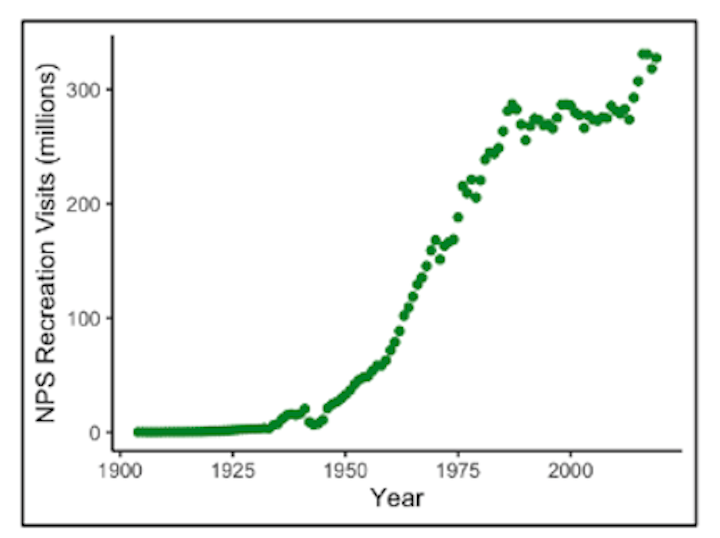
\includegraphics[width=10in]{images/problem_statement_figure_1} \caption{Total annual visitors to the National Park Service system, since its inception through 2020. Visitation has been rapidly increasing, particularly within the last decade. (Source: [IRMA](https://irma.nps.gov/Portal/))}\label{fig:fig1}
\end{figure}

\begin{figure}
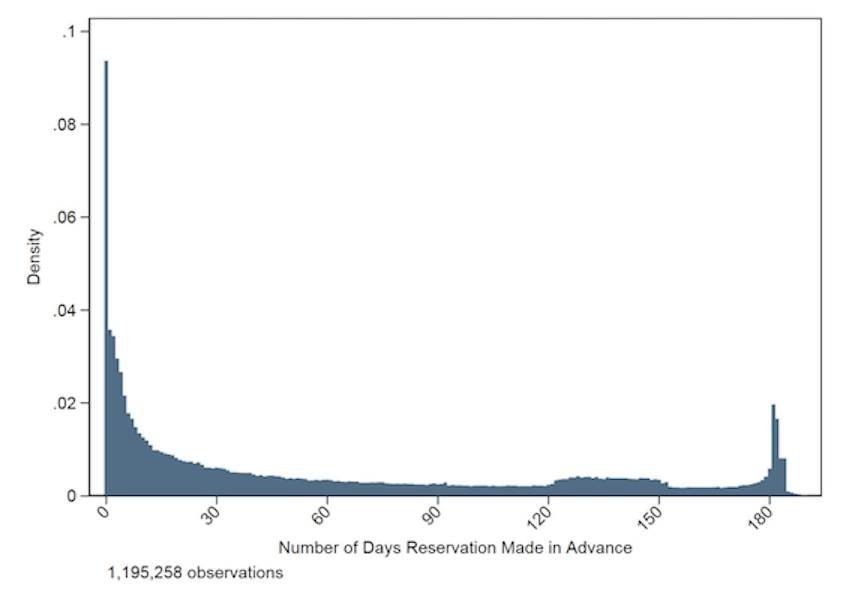
\includegraphics[width=12in]{images/problem_statement_figure_2} \caption{Reproduced from @Walls2018. Days in advance that National Park campsite reservations are made from 2014 to 2016. Reservations are made far in advance, but many reservations are canceled at the last minute.}\label{fig:fig2}
\end{figure}

\begin{figure}
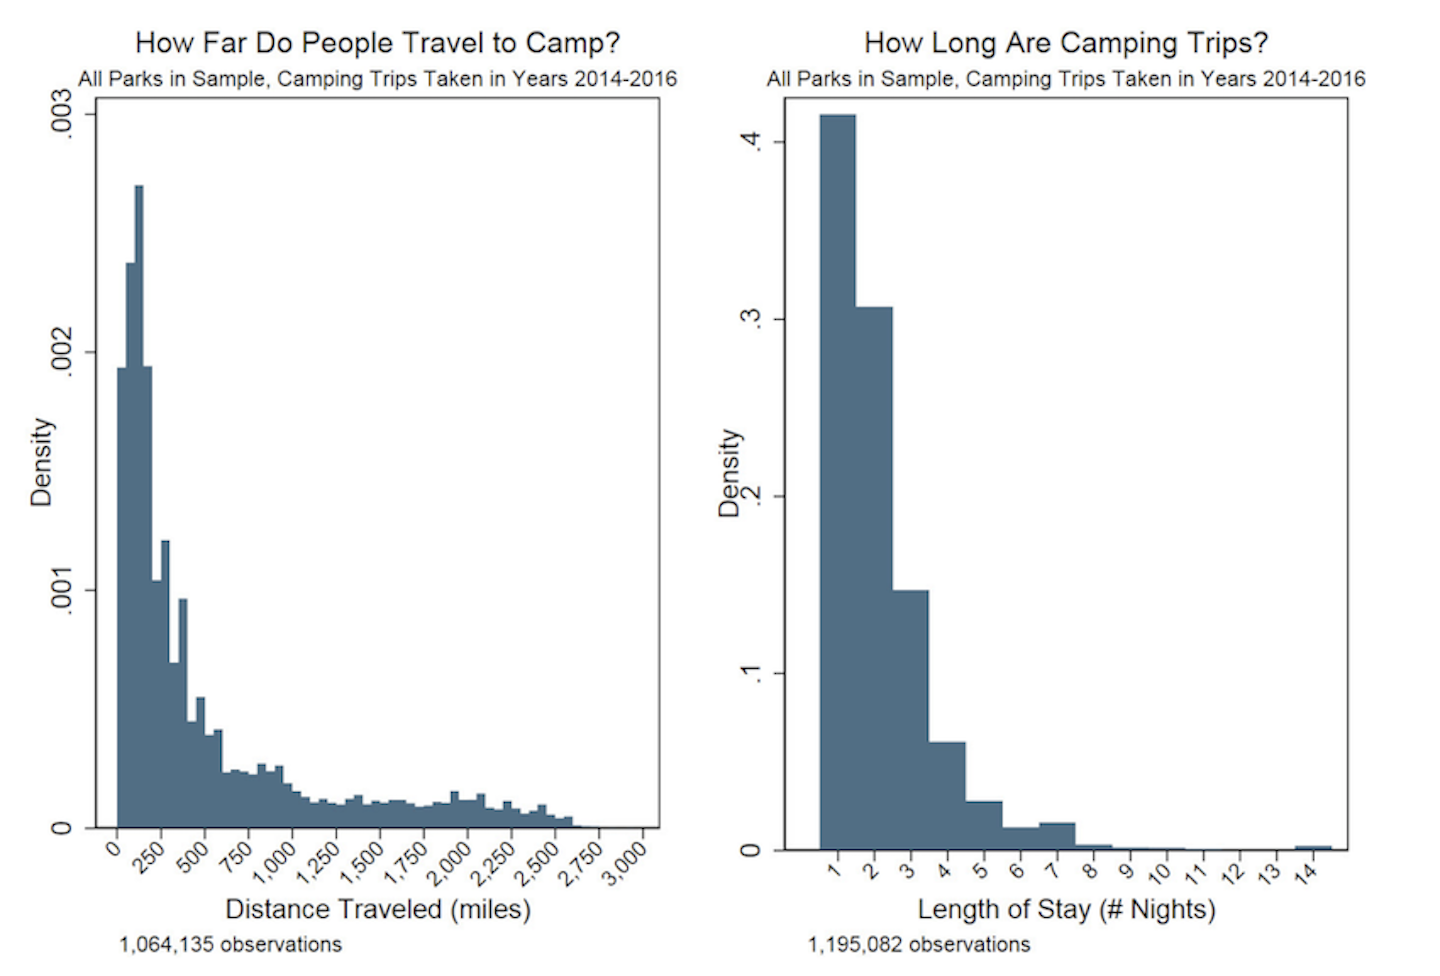
\includegraphics[width=20in]{images/problem_statement_figure_3} \caption{Reproduced from @Walls2018. Distance traveled and duration of stay for National Park camping visits from 2014 to 2016. Visitors tend to visit national parks near their homes and stay only two nights, and longer trips are rare.}\label{fig:fig3}
\end{figure}

\begin{figure}
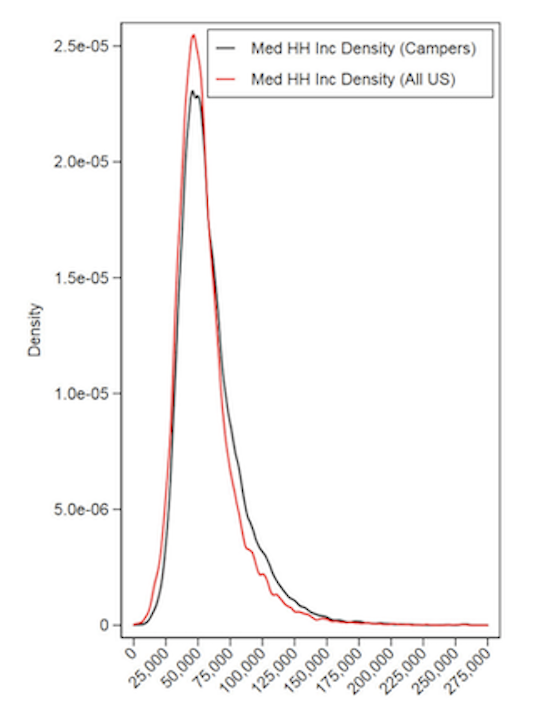
\includegraphics[width=7.78in]{images/problem_statement_figure_4} \caption{Reproduced from @Walls2018. Median household income (by zip code) for National Park campers and for US Population. The black line estimates the distribution of median household (HH) income of campers from 2014 to 2016. The red line estimates the distribution of median household for all zip codes in the U.S. using average median household income from 2014 to 2016 where each zip code is an observation.}\label{fig:fig4}
\end{figure}

\hypertarget{specific-objectives}{%
\chapter{Specific Objectives}\label{specific-objectives}}

Federal lands in the United States provide important recreation opportunities to the public, but there is a \textbf{growing need to understand and mitigate inequities in access to outdoor recreation.} This project addressed this need by creating the \href{https://shinyapps.bren.ucsb.edu/oe_app/}{Outdoor Equity App}, an \textbf{interactive platform} for summarizing and visualizing site-specific patterns and trends in visitation volume, demand, and visitors' location of origin. The platform will integrate nationwide \href{https://www.recreation.gov/}{Recreation.gov} reservation data with \href{https://www.census.gov/data.html}{US census data} to:

\begin{itemize}
\tightlist
\item
  Gain insights into \textbf{demand for reservations} across different types of recreation areas.
\item
  Analyze access to federal public lands among \textbf{historically underserved groups} in
  relation to recreation \textbf{site type, cost, location, and demand}.
\item
  Clearly define all variables and values in the \textbf{metadata documentation}.
\item
  Allow users to \textbf{download a subset of the combined data} for further analysis.
\end{itemize}

\hypertarget{summary-of-solution-design}{%
\chapter{Summary of Solution Design}\label{summary-of-solution-design}}

\hypertarget{glossary-and-definitions}{%
\section{Glossary and Definitions}\label{glossary-and-definitions}}

Throughout this document we define ``reservable sites'' as traditional campgrounds, single remote campsites, overnight boat-in sites or mooring, equestrian sites, cabins, and other shelters listed in the \href{https://ridb.recreation.gov/}{RIDB data}.

\begin{table}

\caption{\label{tab:glossary-table}A table of abbreviations, their definitions, and source URLS.}
\centering
\begin{tabular}[t]{l|l|l}
\hline
Abbreviation & Definition & Source\\
\hline
ACS & American Community Survey & https://www.census.gov/programs-surveys/acs\\
\hline
BLM & Bureau of Land Management & https://www.blm.gov/\\
\hline
BOR & Bureau of Reclamation & https://www.usbr.gov/\\
\hline
MEDS & Master of Environmental Data Science & https://bren.ucsb.edu/masters-programs/master-environmental-data-science\\
\hline
NPS & National Park Service & https://www.nps.gov/index.htm\\
\hline
R1S & Recreation One Stop & https://www.recreation.gov/\\
\hline
UCSB & University of California, Santa Barbara & https://www.ucsb.edu/\\
\hline
USACE & United States Army Corps of Engineers & https://www.usace.army.mil/\\
\hline
USFS & United States Forest Service & https://www.fs.usda.gov/\\
\hline
\end{tabular}
\end{table}

\hypertarget{access-clean-and-wrangle-data}{%
\section{Access, Clean, and Wrangle Data}\label{access-clean-and-wrangle-data}}

\href{https://ridb.recreation.gov/}{RIDB data} and \href{https://www.census.gov/programs-surveys/acs/data.html}{US Census American Communities Survey (ACS) data} are freely available online to the public. We accessed, cleaned, and wrangled all data outside of the \href{https://shinyapps.bren.ucsb.edu/oe_app/}{Outdoor Equity App} using an .Rmd file and 18 custom-made functions (Tables \ref{tab:func-table1}, \ref{tab:func-table2}, \ref{tab:func-table3}, \ref{tab:func-table4}). We downloaded RIDB data in CSV format from Recreation.gov and ACS data through API using the R package \texttt{tidycensus} \citep{R-tidycensus}. We first subsetted RIDB and ACS datasets to include only the variables relevant to our objectives. We then normalized, aggregated, and calculated variables as necessary. Once both datasets are cleaned and wrangled, we joined them using ZIP codes as the key (common value in both datasets). Finally we wrangled the joined RIDB and ACS dataset to ready them for creating data relationship plots.

\begin{table}

\caption{\label{tab:func-table1}A table of the 11 custom cleaning and wrangling functions created for the ACS and RIDB data and the 6 custom cleaning and wrangling functions to create data sets for visitorshed maps and data relationship plots.}
\centering
\begin{tabular}[t]{l|l}
\hline
Script & Purpose\\
\hline
function\_acs\_deciles\_median\_income.R & Calculate decile values of California census household median-income\\
\hline
function\_acs\_education.R & Call and calculate education percentages for given geographic area and state\\
\hline
function\_acs\_language.R & Call and calculate language percentages for given geographic area and state\\
\hline
function\_acs\_median\_income.R & Call and calculate median-income percentages for given geographic area and state\\
\hline
function\_acs\_race.R & Call and calculate race percentages for given geographic area and state\\
\hline
function\_acs\_top\_quartile\_education.R & Calculate weighted third quartile value of California census education percentages\\
\hline
function\_acs\_top\_quartile\_language.R & Calculate weighted third quartile value of California census language percentages\\
\hline
function\_acs\_top\_quartile\_race.R & Calculate weighted third quartile value of California census race percentages\\
\hline
function\_ridb\_subset-pre2018.R & Subset RIDB data\\
\hline
function\_ridb\_variable\_calculate-pre2018.R & Define, standardize, and aggregate values and calculated additional derived variables\\
\hline
function\_join\_ridb\_acs.R & Join RIDB and ACS data\\
\hline
function\_map\_ca\_data.R & Create dataset for California ZIP code visitorshed map\\
\hline
function\_map\_us\_data.R & Create dataset for US State visitorshed map\\
\hline
function\_ridb\_deciles\_median\_income.R & Create dataset for median-income data relationship plots\\
\hline
function\_ridb\_top\_quartile\_education.R & Create dataset for education data relationship plots\\
\hline
function\_ridb\_top\_quartile\_language.R & Create dataset for language data relationship plots\\
\hline
function\_ridb\_top\_quartile\_race.R & Create dataset for race data relationship plots\\
\hline
\end{tabular}
\end{table}

\hypertarget{analysis-and-visualizations}{%
\section{Analysis and Visualizations}\label{analysis-and-visualizations}}

The \href{https://shinyapps.bren.ucsb.edu/oe_app/}{Outdoor Equity App} features interactive maps and plots. Users of this app can select a single reservable site to create custom plots that show a data summary of a single variable or a data relationship between two variables. Visualizations of multiple reservable sites appear as separate plots. Users can also select a single site to create a visitorshed map for the full United States and for the state in which the site is located.

\hypertarget{outdoor-equity-app}{%
\section{Outdoor Equity App}\label{outdoor-equity-app}}

The app has a navigation bar with four tabs: About, Analysis, Metadata and Data Download. Nested under the Analysis tab are the subtabs of Data Summary, Data Relationship, and Visitorshed Maps. The app opens automatically to the About tab.

\begin{figure}
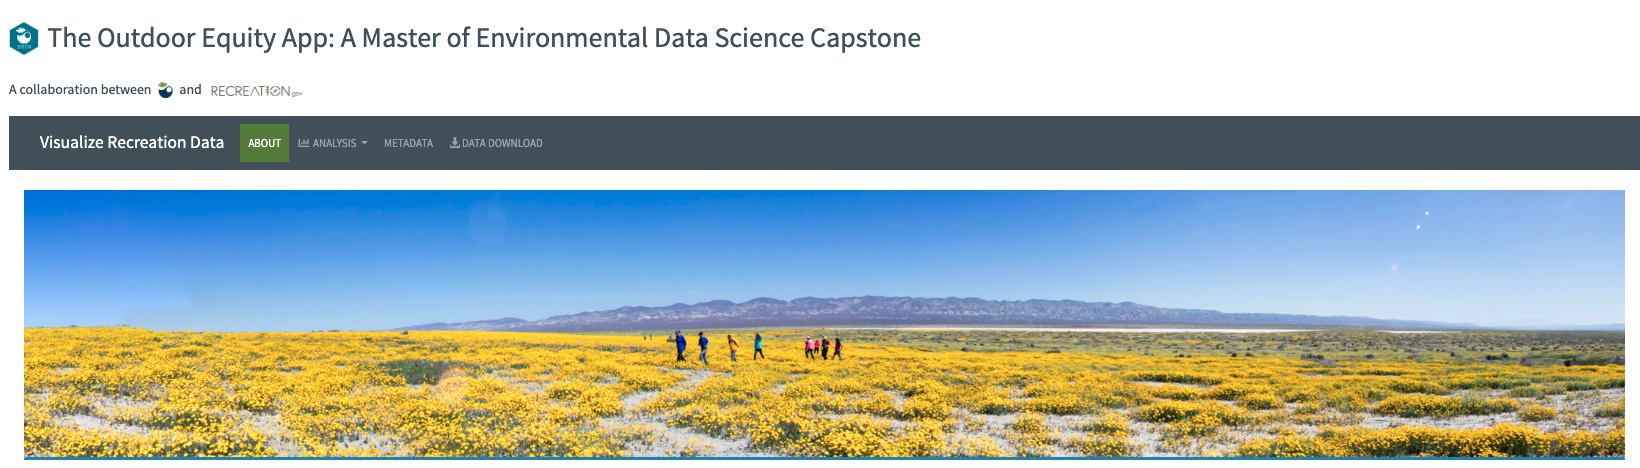
\includegraphics[width=22.78in]{images/screenshot_about} \caption{Screenshot of the About page of the Outdoor Equity App}\label{fig:app-screenshot1}
\end{figure}

\begin{figure}
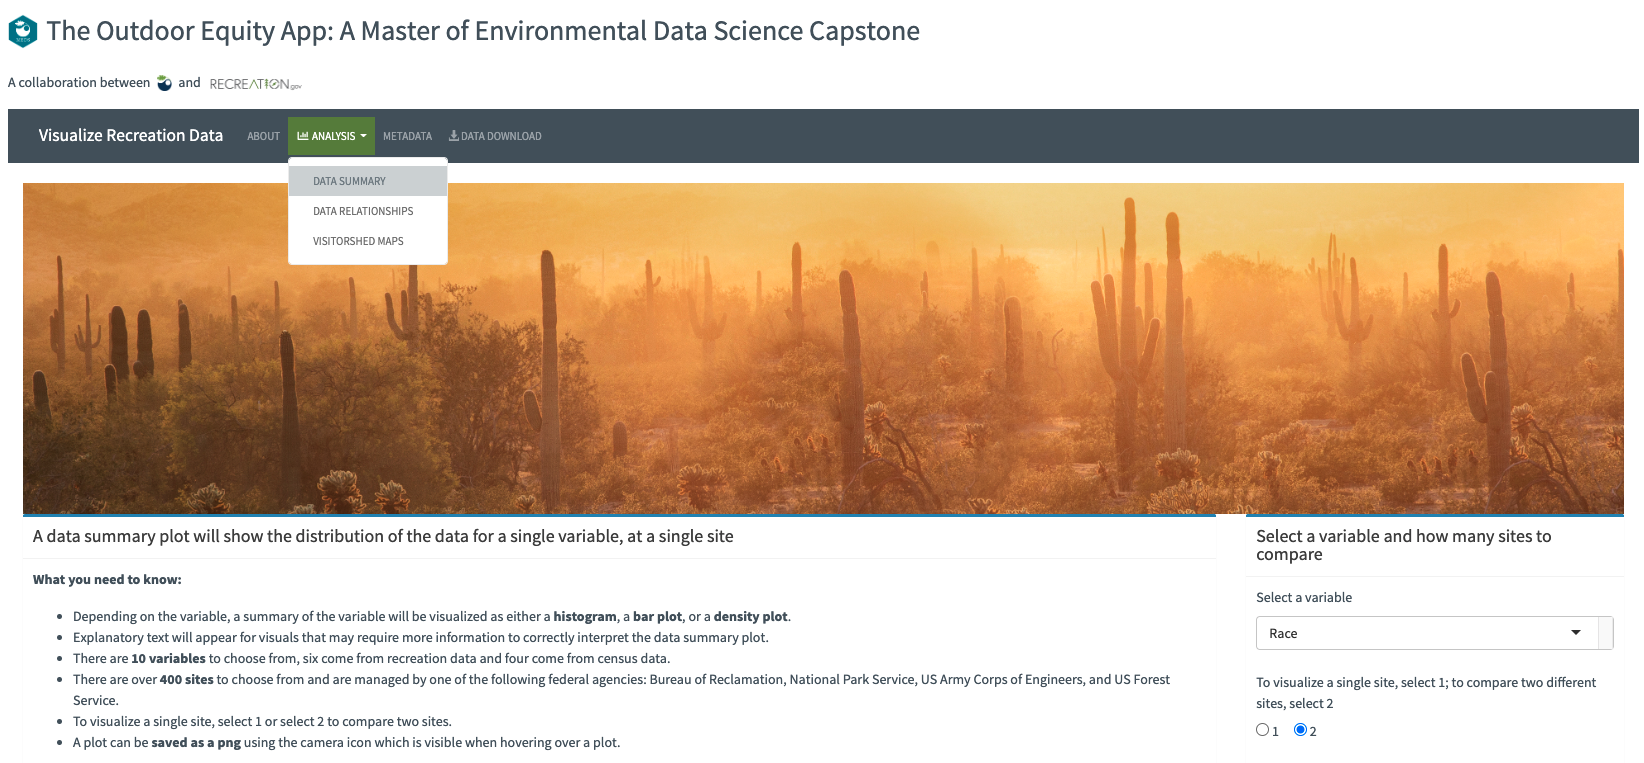
\includegraphics[width=22.83in]{images/screenshot_data-summary} \caption{Screenshot of the Analysis page of the Outdoor Equity App}\label{fig:app-screenshot2}
\end{figure}

\begin{figure}
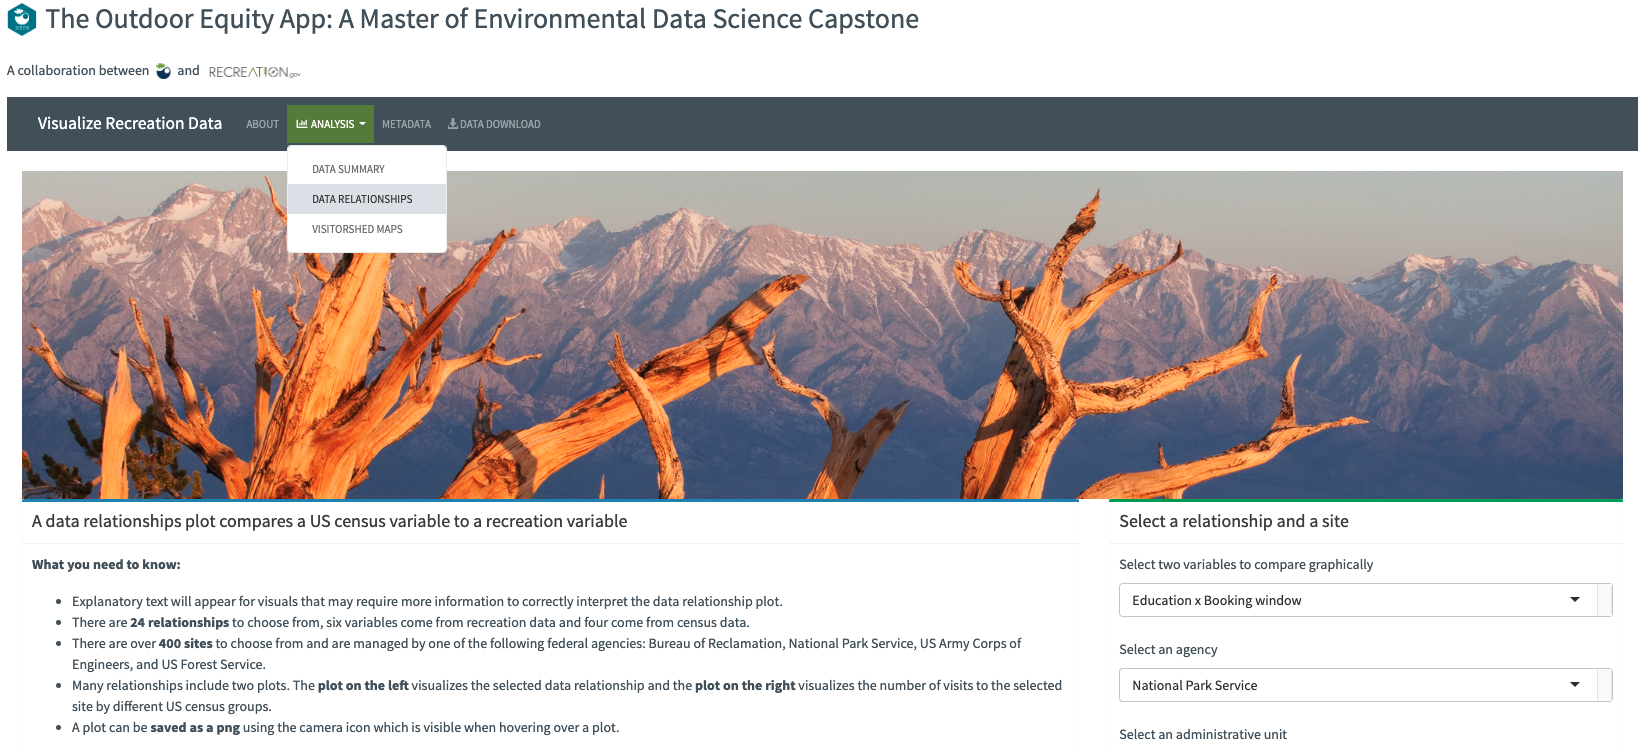
\includegraphics[width=22.78in]{images/screenshot_data-relationship} \caption{Screenshot of the Analysis page of the Outdoor Equity App}\label{fig:app-screenshot3}
\end{figure}

\begin{figure}
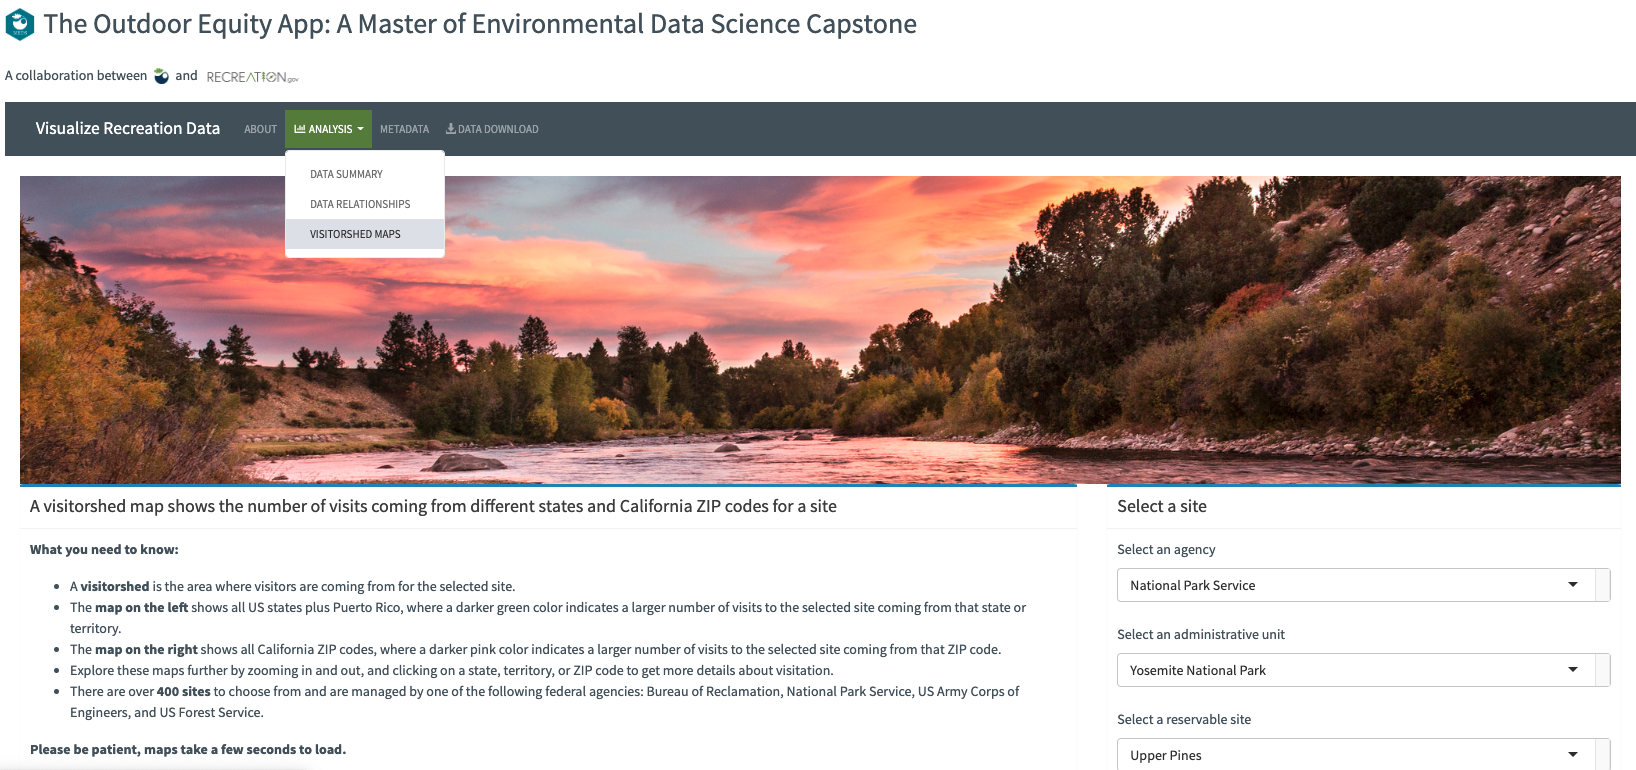
\includegraphics[width=22.72in]{images/screenshot_visitorshed} \caption{Screenshot of the Analysis page of the Outdoor Equity App}\label{fig:app-screenshot4}
\end{figure}

\begin{figure}
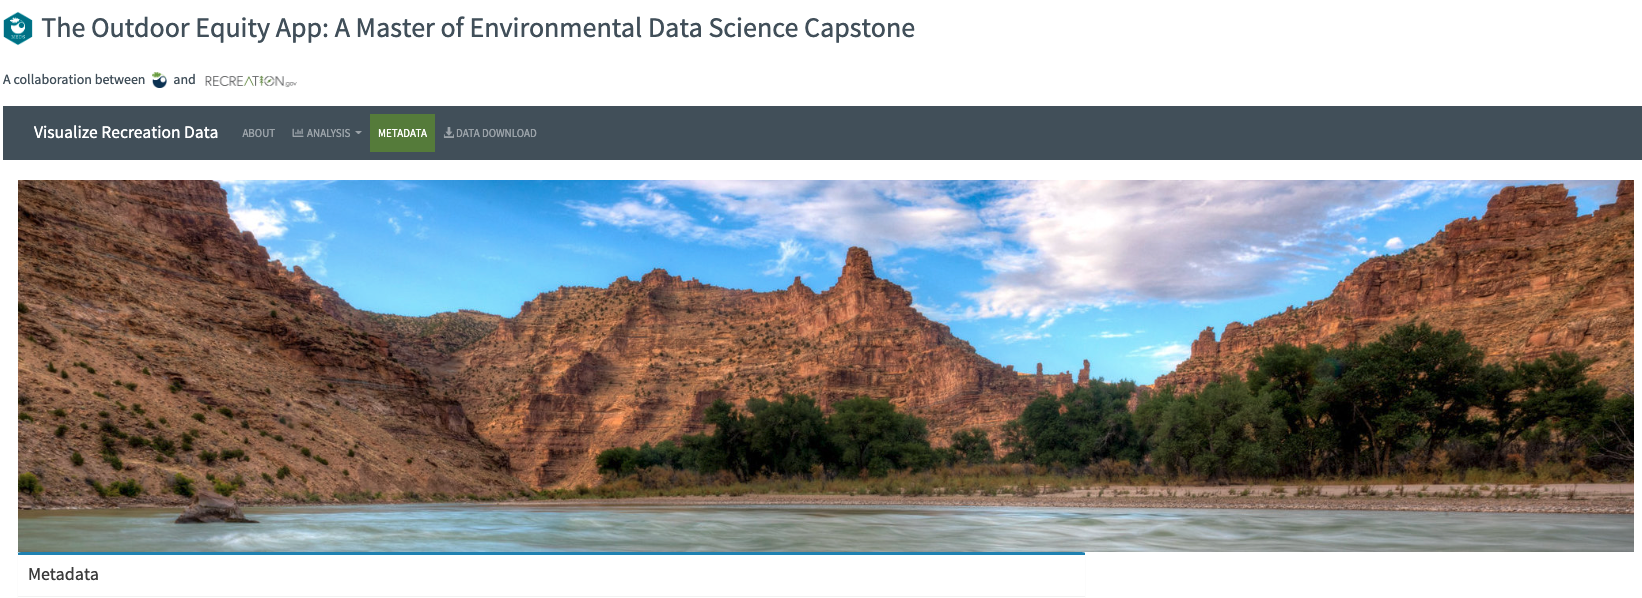
\includegraphics[width=22.81in]{images/screenshot_metadata} \caption{Screenshot of the Metadata page of the Outdoor Equity App}\label{fig:app-screenshot5}
\end{figure}

\begin{figure}
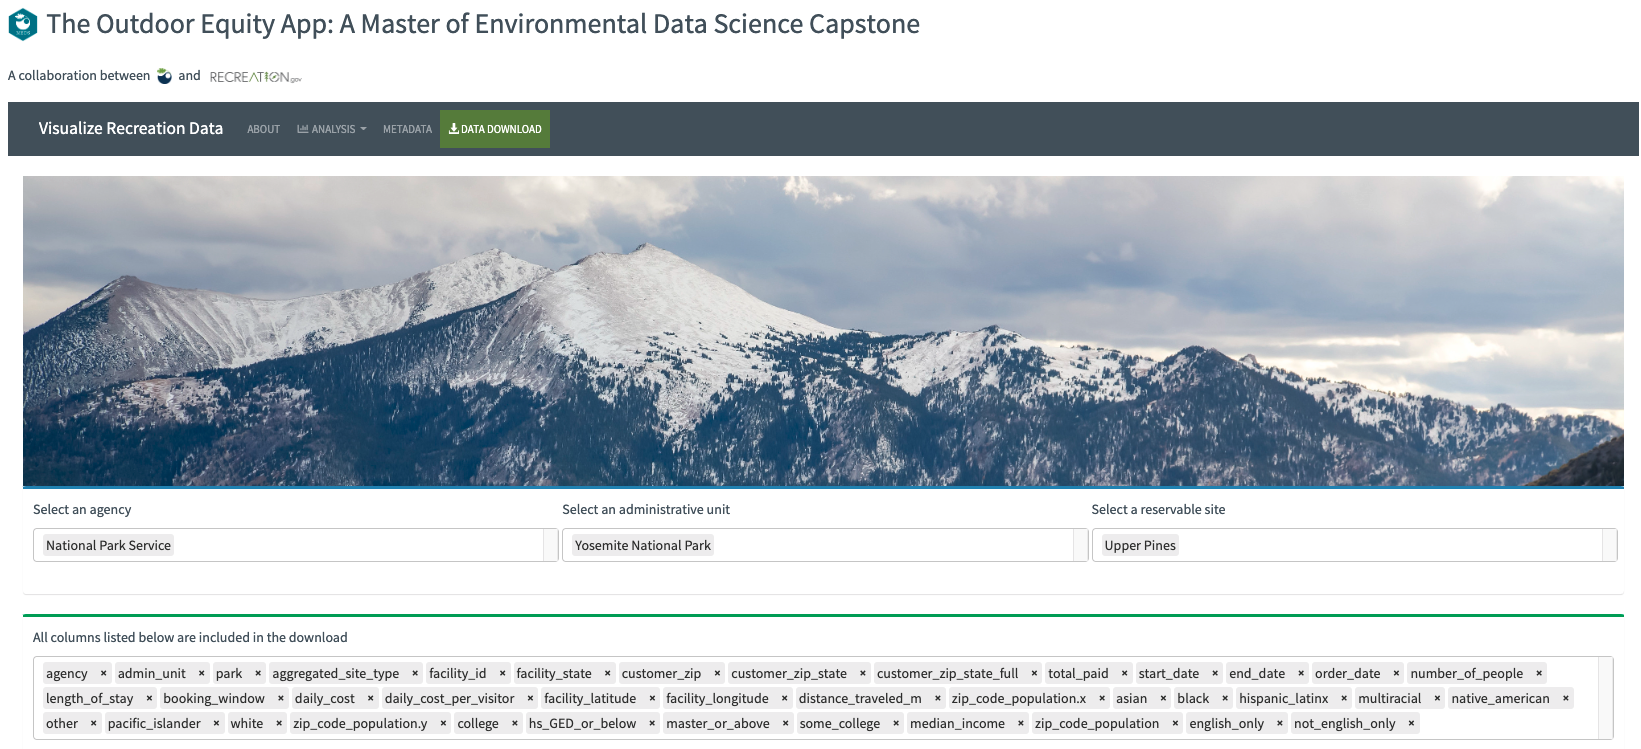
\includegraphics[width=22.79in]{images/screenshot_data-download} \caption{Screenshot of the Metadata page of the Outdoor Equity App}\label{fig:app-screenshot6}
\end{figure}

\hypertarget{user-guide-and-technical-documentation}{%
\section{User Guide and Technical Documentation}\label{user-guide-and-technical-documentation}}

The \href{https://shinyapps.bren.ucsb.edu/oe_app/}{Outdoor Equity App} includes a user guide and metadata information. The user guide section includes a quick overview of the app and helper text on how to start creating visuals.

This technical documentation is created with the \texttt{bookdown} package \citep{R-bookdown} and is linked in the About tab of the Outdoor Equity App. Metadata for all variables used within the app are also available on the app Metadata tab and in the \protect\hyperlink{products-and-deliverables}{Products and Deliverables Section} of this document.

\hypertarget{products-and-deliverables}{%
\chapter{Products and Deliverables}\label{products-and-deliverables}}

\hypertarget{r-shiny-app}{%
\section{R Shiny App}\label{r-shiny-app}}

The Outdoor Equity Shiny App has the following functionality:

\begin{itemize}
\tightlist
\item
  Visualize statistical distributions of RIDB and US Census variables
\item
  Visualize relationships between RIDB and US census variables
\item
  Created visualizations can be downloaded as png
\item
  View visitorshed maps of reservable sites both nationally and within state site is located in
\item
  Download customized subsets of the data
\end{itemize}

Help documentation:

\begin{itemize}
\tightlist
\item
  User guide
\item
  Metadata
\item
  Background
\end{itemize}

\hypertarget{metadata}{%
\section{Metadata}\label{metadata}}

\begin{verbatim}
## Rows: 38 Columns: 9-- Column specification --------------------------------------------------------
## Delimiter: ","
## chr (7): variable name, data_source, definition, unit, class, data_type, pro...
## dbl (1): total_unique_values
## lgl (1): missing_value_code
## i Use `spec()` to retrieve the full column specification for this data.
## i Specify the column types or set `show_col_types = FALSE` to quiet this message.
\end{verbatim}

\begin{Shaded}
\begin{Highlighting}[]
\CommentTok{\# create table of metadata}
\NormalTok{knitr}\SpecialCharTok{::}\FunctionTok{kable}\NormalTok{(data\_joined\_2018\_metadata\_df,}
             \AttributeTok{align =} \StringTok{"l"}\NormalTok{,}
             \AttributeTok{caption =} \StringTok{"Metadata of joined RIDB{-}ACS dataset"}\NormalTok{,}
             \AttributeTok{row.names =} \ConstantTok{FALSE}\NormalTok{)}
\end{Highlighting}
\end{Shaded}

\begin{table}

\caption{\label{tab:unnamed-chunk-4}Metadata of joined RIDB-ACS dataset}
\centering
\begin{tabular}[t]{l|l|l|l|l|l|l|l|l}
\hline
variable name & data\_source & definition & unit & class & data\_type & provenance (which scripts if used to created this var) & missing\_value\_code & total\_unique\_values\\
\hline
agency & ridb & NA & NA & character & categorical & none & NA & 4\\
\hline
admin\_unit & ridb & NA & NA & character & categorical & none & NA & 43\\
\hline
park & ridb & NA & NA & character & categorical & none & NA & 447\\
\hline
aggregated\_site\_type & ridb & NA & NA & character & categorical & data\_preparation/functions/function\_ridb\_variable\_calculate-pre2018.R & NA & 7\\
\hline
facility\_id & ridb & NA & NA & NA & NA & NA & NA & NA\\
\hline
facility\_state & ridb & NA & NA & character & categorical & none & NA & 1\\
\hline
customer\_zip & ridb & NA & NA & character & categorical & none & NA & 15861\\
\hline
customer\_zip\_state & acs & NA & NA & NA & NA & NA & NA & NA\\
\hline
customer\_zip\_state\_full & acs & NA & NA & NA & NA & NA & NA & NA\\
\hline
total\_paid & ridb & NA & NA & numeric & NA & NA & NA & 1567\\
\hline
start\_date & ridb & NA & NA & date & NA & NA & NA & 734\\
\hline
end\_date & ridb & NA & NA & date & NA & NA & NA & 731\\
\hline
order\_date & ridb & NA & NA & date & NA & NA & NA & 364\\
\hline
number\_of\_people & ridb & NA & NA & numeric & NA & none & NA & 80\\
\hline
length\_of\_stay & ridb & NA & NA & numeric & NA & NA & NA & 21\\
\hline
booking\_window & ridb & NA & NA & numeric & NA & NA & NA & 444\\
\hline
daily\_cost\_per\_visitor & ridb & NA & NA & numeric & NA & NA & NA & 5095\\
\hline
facility\_latitude & ridb & NA & NA & NA & NA & none & NA & NA\\
\hline
facility\_longitude & ridb & NA & NA & NA & NA & none & NA & NA\\
\hline
distance\_traveled\_m & ridb & NA & NA & numeric & NA & NA & NA & NA\\
\hline
zip\_code\_population.x & acs & NA & NA & NA & NA & NA & NA & NA\\
\hline
asian & acs & NA & NA & numeric & NA & NA & NA & NA\\
\hline
black & acs & NA & NA & numeric & NA & NA & NA & NA\\
\hline
hispanic\_latinx & acs & NA & NA & numeric & NA & NA & NA & NA\\
\hline
multiracial & acs & NA & NA & numeric & NA & NA & NA & NA\\
\hline
native\_american & acs & NA & NA & numeric & NA & NA & NA & NA\\
\hline
other & acs & NA & NA & numeric & NA & NA & NA & NA\\
\hline
pacific\_islander & acs & NA & NA & numeric & NA & NA & NA & NA\\
\hline
white & acs & NA & NA & numeric & NA & NA & NA & NA\\
\hline
zip\_code\_population.y & acs & NA & NA & NA & NA & NA & NA & NA\\
\hline
college & acs & estimated percentage of population with a college degree in a zip code & percentage & numeric & continuous & data\_preparation/functions/function\_acs\_education.R & NA & 11641\\
\hline
hs\_GED\_or\_below & acs & estimated percentage of population with a high school General Educational Development (GED) degree or below in a zip code & percentage & numeric & continuous & data\_preparation/functions/function\_acs\_education.R & NA & 11705\\
\hline
master\_or\_above & acs & estimated percentage of population with a master degree or above in a zip code & percentage & numeric & continuous & data\_preparation/functions/function\_acs\_education.R & NA & 11445\\
\hline
some\_college & acs & estimated percentage of population with some college education in a zip code & percentage & numeric & continuous & data\_preparation/functions/function\_acs\_education.R & NA & 11631\\
\hline
median\_income & acs & median household income in the past 12 months in 2019 inflation-adjusted dollars & dollars & numeric & continuous & data\_preparation/functions/function\_acs\_median\_income.R & NA & 10439\\
\hline
zip\_code\_population & acs & NA & NA & numeric & NA & NA & NA & NA\\
\hline
english\_only & acs & estimated percentage of population that speak only english in the home in a zip code & percentage & numeric & continuous & data\_preparation/functions/function\_acs\_language.R & NA & 11469\\
\hline
not\_english\_only & acs & estimated percentage of population that speak a language other than english in the home in a zip code & percentage & numeric & continuous & data\_preparation/functions/function\_acs\_language.R & NA & 11469\\
\hline
\end{tabular}
\end{table}

\hypertarget{summary-of-testing}{%
\chapter{Summary of Testing}\label{summary-of-testing}}

\hypertarget{data-integrity}{%
\section{Data Integrity}\label{data-integrity}}

We screened the data for outliers by summarizing and visualizing the raw data, and assessed whether those outliers need to be removed. We consulted other researchers who are familiar with the RIDB datasets to confirm outliers or other anomalies in the data.

Additionally, we documented the percent loss from data wrangling to ensure that our cleaning and wrangling of the data were reasonable.

\hypertarget{code-review}{%
\section{Code Review}\label{code-review}}

We conducted code reviews within the team, and with faculty or external advisers. We reviewed specific code chunks and scripts related to the Outdoor Equity App.

We separated our workflows so that one person created scripts, and the other reviewed them. We did this to maintain some objectivity when evaluating if our datasets were aggregating correctly. We also had a separate workflow for metadata, where one person created and wrote metadata, and the other reviewed it. This confirmed that the data matches how it is being described in the metadata. This confirmation is important as we want our client to be able to scale our product and workflows for future use.

\hypertarget{product-testing}{%
\section{Product Testing}\label{product-testing}}

We used three packages to test our R Shiny app. We used \texttt{shinytest} to ensure our app is visualized the way we expect it to using the package's snapshot-based testing strategy. We used \texttt{shinyloadtest} to test the server hosting the R Shiny App to ensure that it responds in a reasonable amount of time based on the inputs a user provides. Similarly, we utilized the \texttt{tictoc} package during our data wrangling and cleaning, and when we initially created our plots, graphs, and maps to estimate an informed guess of how long it may take the app to run our scripts. Lastly, we used the \texttt{reactlog} package's diagnostic tool which creates a reactive visualizer for the app to make sure that reactive elements are working the way we expected them to. It is important to note that this diagnostic tool was not useful as our app functionality increased, as the reactive visualizer became impossible to read. There may be other options within \texttt{reactlog} to use the reactive visualizer in a different way, but we did not have enough time to research this.

We added temporary print statements to all functions in the app to ensure that the functions were working correctly were are outputting what we expect. We removed print statements from functions that were functioning with zero errors. We did this because print statements can take a long time to run and should not be left in functions or in the app permanently.

Additionally, we held multiple meetings with the Recreation One Stop team to obtain real-time and focused feedback to improve user design and experience.

\hypertarget{next-steps-for-testing}{%
\subsection{Next steps for testing}\label{next-steps-for-testing}}

Due to time constraints, we were not able to implement all testing methods we wanted. We recommend the following testing strategies to make the app more robust and for smoother functionality.

\begin{itemize}
\tightlist
\item
  Use the R package \texttt{testthat} to conduct unit tests on the scripts used to create Tidy datasets and for subsetted datasets for visualization. This type of testing may be important to avoid silent failures and to ensure that the datasets are aggregating correctly.
\item
  Use \texttt{gremlin.js}, a JavaScript library used for ``Monkey testing'' to test the behavior of the R Shiny App. This package is compatible with \texttt{shiny} and does not require any external installation. ``Monkey testing'' is a type of testing where random, automated tests provide random inputs and then checks the behavior of the app (i.e.~if the system or application crashes). We were able to find some finicky bugs through our own testing of random inputs, but ``Monkey testing'' is the formal process.
\item
  Employ user testing with federal public land managers, researchers, and those who are not familiar with RIDB data to further enhance the user experience and design.
\end{itemize}

\hypertarget{user-documentation}{%
\chapter{User Documentation}\label{user-documentation}}

\hypertarget{purpose-of-the-outdoor-equity-application}{%
\section{Purpose of the Outdoor Equity Application}\label{purpose-of-the-outdoor-equity-application}}

\hypertarget{how-to-use-the-outdoor-equity-app}{%
\section{How to Use the Outdoor Equity App}\label{how-to-use-the-outdoor-equity-app}}

\hypertarget{about-the-app}{%
\subsection{About the APP}\label{about-the-app}}

\hypertarget{metadata-1}{%
\subsection{Metadata}\label{metadata-1}}

\hypertarget{data-summary}{%
\subsection{Data Summary}\label{data-summary}}

\hypertarget{data-relationships}{%
\subsection{Data Relationships}\label{data-relationships}}

\hypertarget{visitorshed-maps}{%
\subsection{Visitorshed Maps}\label{visitorshed-maps}}

\hypertarget{data-download}{%
\subsection{Data Download}\label{data-download}}

\hypertarget{how-to-maintain-the-outdoor-equity-app}{%
\section{How to Maintain the Outdoor Equity App}\label{how-to-maintain-the-outdoor-equity-app}}

\hypertarget{data-preparation-methods}{%
\subsection{Data Preparation Methods}\label{data-preparation-methods}}

\hypertarget{ridb-data}{%
\subsubsection{RIDB Data}\label{ridb-data}}

\hypertarget{u.s.-census-data}{%
\subsubsection{U.S. Census Data}\label{u.s.-census-data}}

\hypertarget{data-joining}{%
\subsubsection{Data Joining}\label{data-joining}}

\hypertarget{statistical-analysis-and-data-wrangling-for-plots}{%
\subsection{Statistical Analysis and Data Wrangling for Plots}\label{statistical-analysis-and-data-wrangling-for-plots}}

\hypertarget{data-summary-1}{%
\subsubsection{Data Summary}\label{data-summary-1}}

\hypertarget{data-relationships-1}{%
\subsubsection{Data Relationships}\label{data-relationships-1}}

\hypertarget{spatial-analysis}{%
\subsubsection{Spatial analysis}\label{spatial-analysis}}

\hypertarget{data-limitations}{%
\subsection{Data Limitations}\label{data-limitations}}

\hypertarget{data-updates}{%
\subsection{Data updates}\label{data-updates}}

\hypertarget{server-hosting}{%
\subsection{Server Hosting}\label{server-hosting}}

\hypertarget{shiny-code-directory}{%
\subsection{Shiny Code Directory}\label{shiny-code-directory}}

\hypertarget{how-to-expand-the-outdoor-equity-app}{%
\section{How to Expand the Outdoor Equity App}\label{how-to-expand-the-outdoor-equity-app}}

\hypertarget{temporal-expansions}{%
\subsection{Temporal Expansions}\label{temporal-expansions}}

\hypertarget{spatial-expansions}{%
\subsection{Spatial Expansions}\label{spatial-expansions}}

\hypertarget{statistical-analysis}{%
\subsection{Statistical Analysis}\label{statistical-analysis}}

\hypertarget{additional-challenges}{%
\chapter{Additional Challenges}\label{additional-challenges}}

\hypertarget{archive-access}{%
\chapter{Archive Access}\label{archive-access}}

  \bibliography{book.bib,packages.bib}

\end{document}
